\documentclass[xcolor=dvipsnames]{beamer}

\usepackage{amsmath, amssymb, graphicx}
\usepackage[english]{babel}
\usepackage{times}
\usepackage[utf8]{inputenc}
\usepackage[T1]{fontenc}
\usepackage{listings}
\usepackage{hyperref}
\usepackage[norelsize,ruled,vlined]{algorithm2e}
\usepackage{color}
\usepackage{hyperref}
\usepackage{booktabs}
\usepackage{tikz}
\usetikzlibrary{matrix}
\usetikzlibrary{arrows}
\usetikzlibrary{positioning}
\usetikzlibrary{shapes.multipart}

\theoremstyle{definition}
\newtheorem{proposition}{Proposition}

\mode<presentation>
\usecolortheme{fly}

\setbeamercolor{alerted text}{fg=purple}

\setbeamertemplate{footline}{%
  \usebeamercolor[fg]{navigation symbols}%
  \usebeamerfont{footline}
  \parbox{\linewidth}{
    \vspace*{-8pt}
    \hspace{5pt}\insertpagenumber/\inserttotalframenumber
    %% \insertshortauthor\hspace{5pt}\insertshortinstitute
    %% \hfill \insertsection
    %% \hfill\usebeamertemplate***{navigation symbols}
    %% \hfill
  }
}
%% \setbeamertemplate{navigation symbols}{}

\lstset{language = [LaTeX]TeX,
    % captionpos=b,
    basicstyle= \small \ttfamily,
    keywordstyle = \bfseries \color{blue},
    commentstyle = \color{green}
}

\title[Free Will Is Creative]{Free Will Is Creative\\
{\small Towards A New Conception of Free Will}
}
\author{Fengyun Liu}
\institute[EPFL]{EPFL}
\date{\today}


% Delete this, if you do not want the table of contents to pop up at
% the beginning of each subsection:
%% \AtBeginSection[]
%% {\begin{frame}<beamer>{Overview}
%%         \tableofcontents[
%%             sections={1-6},
%%             currentsection,
%%             currentsubsection,
%%             hideothersubsections,
%%             sectionstyle=show/shaded,
%%         subsectionstyle=show/shaded/hide]
%%     \end{frame}
%% }

\begin{document}


%%%%%%%%%%%%%%%%%%%%%%%%%%%%%%%%%%%%%%%%%%%%%%%%%%%%%%%%%%%%%%%
% 0. Titlepage
%%%%%%%%%%%%%%%%%%%%%%%%%%%%%%%%%%%%%%%%%%%%%%%%%%%%%%%%%%%%%%%
\begin{frame}
    \titlepage{}
\end{frame}
\begin{frame}{Today's agenda}
\tableofcontents[hideallsubsections,
    sections={1-6}
]
\end{frame}

%%%%%%%%%%%%%%%%%%%%%%%%%%%%%%%%%%%%%%%%%%%%%%%%%%%%%%%%%%%%%%%
% 1. Background
%%%%%%%%%%%%%%%%%%%%%%%%%%%%%%%%%%%%%%%%%%%%%%%%%%%%%%%%%%%%%%%
% subsection Motivation (end)
\section{Traditional View of Free Will} % (fold)
\label{sec:Background}

\begin{frame}[fragile]
  \frametitle{Free Will as the Capacity to Choose}
  Traditional philosophers characterize free will as the \alert{capacity to choose}.

  \begin{itemize}
  \item Libertarians: \emph{The ability to do otherwise}
  \item Compatibilists: \emph{The ability to align desires and actions}
  \end{itemize}
\end{frame}

\begin{frame}[fragile]
  \frametitle{The Magic Power of Choice}
  An agent has free will can do either A or B, solely based on his/her choice.

  \begin{figure}
    \centering
    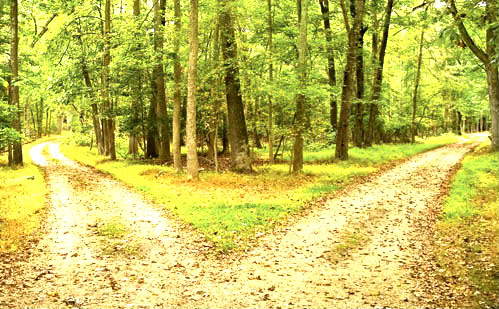
\includegraphics[width=0.8\textwidth]{images/woods.jpg}\\
    \emph{Two Roads Diverged In a Yellow Wood}
  \end{figure}
\end{frame}

\begin{frame}[fragile]
  \frametitle{The Magic Power of Choice}
  Once owned this magic power, it can be used \alert{anywhere}, \alert{anytime} and on \alert{any matters}.
  \begin{figure}
    \centering
    
\includegraphics[width=0.8\textwidth]{images/magic.jpg}\\
  \end{figure}
\end{frame}


%%%%%%%%%%%%%%%%%%%%%%%%%%%%%%%%%%%%%%%%%%%%%%%%%%%%%%%%%%%%%%%
% 2. The Myth of Choice
%%%%%%%%%%%%%%%%%%%%%%%%%%%%%%%%%%%%%%%%%%%%%%%%%%%%%%%%%%%%%%%
\section{The Myth of Choice} % (fold)
\label{sec:myth}

\begin{frame}[fragile]
  \frametitle{The Myth of Choice}
  I dub the view of \emph{free will as the magic power of choice} as the \alert{myth of choice}.\\[1cm]

  Tasks of this presentation:
  \begin{itemize}
  \item Break the \emph{myth of choice}
  \item Show that \emph{free will is creative}
  \end{itemize}
\end{frame}


%%%%%%%%%%%%%%%%%%%%%%%%%%%%%%%%%%%%%%%%%%%%%%%%%%%%%%%%%%%%%%%
% 3. Free Will is Creative
%%%%%%%%%%%%%%%%%%%%%%%%%%%%%%%%%%%%%%%%%%%%%%%%%%%%%%%%%%%%%%%
\section{Free Will is Creative} % (fold)
\label{sec:creative}

%%%%%%%%%%%%%%%%%%%%%%%%%%%%%%%%%%%%%%%%%%%%%%%%%%%%%%%%%%%%%%%
% 4. Conclustion
%%%%%%%%%%%%%%%%%%%%%%%%%%%%%%%%%%%%%%%%%%%%%%%%%%%%%%%%%%%%%%%
\section{Conclusion} % (fold)
\label{sec:conclusion}

\end{document}
